\chapter{Self-Drive}

A skill becomes serious only when life begins to demand it.

Before that moment, the skill may be admired. It may be praised. It may appear on a plan, a wish list, a New Year's resolution, or a course receipt. But admiration is not necessity. A person can admire English, investing, writing, exercise, programming, sales, public speaking, or clear thinking for many years and still remain almost unchanged.

The common explanation is that such people lack willpower. That explanation is usually too shallow. Willpower is visible at the surface, but the deeper question is this:

\begin{quote}
Has this skill become a real necessity in this person's life?
\end{quote}

If not, the result is predictable. The person will postpone, restart, complain, search for better methods, buy more tools, and then stop again. He may sincerely believe the skill is important, but importance alone does not move him. Necessity moves him.

Self-drive is not a mysterious inner flame. It is the mind's response to a chosen necessity. When something becomes necessary enough, the person does not wait for a perfect mood. He uses the skill awkwardly, then repeatedly, then better. He solves problems as they appear because the work has entered his actual life.

\section*{The English Example}

Many educated people have spent years studying English and still cannot use it comfortably. Six years in primary school, three years in middle school, three years in high school, four years in university, sometimes even more, and yet listening, speaking, reading, and writing remain weak.

This cannot be explained by intelligence alone. Acquiring a language does not require exceptional intelligence. In multilingual regions, many ordinary people naturally use more than one language. Children do it. Adults do it. People with no special academic talent do it. Even household commands can be learned across languages when the environment repeatedly requires response.

So the serious question is not, ``Why is English so hard?''

The better question is:

\begin{quote}
For most learners, what was the real necessity?
\end{quote}

For many people, the necessity was not using English. The necessity was passing English exams. Once the exams ended, the need disappeared. The person had not built a life in which English was used to read, work, think, trade, travel, learn, or communicate. English was a gate to pass through, not a tool to live with.

This explains a great deal. A person may say, ``English is important,'' because everyone around him says it. But if his daily life is not damaged by poor English, and if better English would not immediately open any path he cares about, the brain receives a different message: this is optional.

Optional things are easy to abandon.

The few who do learn differently usually have a different relation to the skill. They need it. They may need it to read the best material in their field. They may need it to serve customers, talk with colleagues, study documentation, apply for work, or enter a market. The stronger the need, the faster the learning. Even before they are good, they use it. By using it badly, they create the conditions for using it better.

This is the hidden law:

\begin{quote}
A skill improves fastest when it is pulled into life before it is fully ready.
\end{quote}

\section*{Use Creates Demand}

The word ``learn'' is often misleading. People imagine learning as preparation for a future use. In many cases, the order must be reversed. Begin using, and the pressure of use teaches you what to learn next.

A person who loves reading may decide that nonfiction books should be read in the original language whenever possible. At that moment, English reading stops being a school subject. It becomes a way to feed the mind. The difficulty is still there. Unknown words still appear. Sentences are still slow. But the friction no longer decides the outcome, because the desire to finish the book is stronger than the discomfort of reading it.

The same person may still speak English poorly, because speaking is not equally necessary in his life. This is not a contradiction. Necessity is specific. ``English'' is too broad a category. English reading, English speaking, English writing, and English listening may each have different degrees of necessity.

This distinction matters in every field. A person may want to ``learn investing,'' but what is the real use? Reading annual reports? Understanding risk? Controlling greed? Holding cash? Writing an investment thesis? Avoiding leverage? Each subskill becomes real only when it is attached to an actual decision.

A person may want to ``learn writing,'' but what is the real use? Clarifying his own thought? Selling a product? Building a reputation? Teaching a team? Recording principles? If writing is only a romantic identity, it remains fragile. If writing becomes the instrument through which he earns trust, thinks clearly, and compounds influence, it becomes much harder to abandon.

\section*{The Necessity Test}

When a desired skill keeps failing to appear, do not begin by blaming laziness. Begin by testing whether the skill has any consequence in life.

\begin{center}
\begin{adjustbox}{max width=\linewidth}
\begin{tabular}{p{0.24\linewidth}p{0.31\linewidth}p{0.31\linewidth}}
\hline
 & Short term & Long term \\
\hline
Useful & What does it improve now? & What does it compound later? \\
Not useful & What comfort does it merely decorate? & What fantasy does it merely support? \\
\hline
\end{tabular}
\end{adjustbox}
\end{center}

This table is deliberately simple. Put the skill into it honestly.

If a skill is useful neither now nor later, it is probably not a real goal. It may be a borrowed desire. If it is useful only as decoration, it will lose to comfort. If it compounds later but has no present use, you must design a present use for it. Otherwise the future benefit will remain too abstract to drive behavior.

The practical question is:

\begin{quote}
How can I make this skill part of my normal life before I become good at it?
\end{quote}

Do not wait until you can read perfectly before reading. Do not wait until you can write well before writing. Do not wait until you understand markets perfectly before learning how to record decisions and manage risk with small amounts. Do not wait until you are persuasive before trying to sell something modest. Use creates feedback. Feedback creates correction. Correction creates growth.

Waiting creates only a better excuse.

\section*{Analysis as a Necessity}

Some people seem naturally analytical. They keep asking why. They are not satisfied with a surface explanation. They observe, compare, test, summarize, revise, and then begin again. When they encounter a problem that deserves an explanation, they may think about it for months or years. Their conclusion improves because the question keeps living in their mind.

This is not merely a talent. It is a necessity.

For such people, truth has weight. Not understanding is uncomfortable. A loose explanation feels unfinished. A contradiction irritates them. A better model gives them genuine pleasure. Therefore they keep going when others stop.

This is one reason they can become independent and right. They do not analyze only after trouble has arrived. They analyze before trouble arrives. They do not wait for reality to punish them. They try to understand the structure early enough to choose better.

Analysis may be the king of abilities because it improves other abilities. It helps a person learn, choose, invest, sell, negotiate, build, write, and correct himself. Yet formal education often fails to cultivate it deeply. Many people pass exams without becoming good at analysis. The minority who acquire it usually do so because they cannot tolerate confusion for long.

Their loop looks like this:

\begin{center}
\begin{adjustbox}{max width=\linewidth}
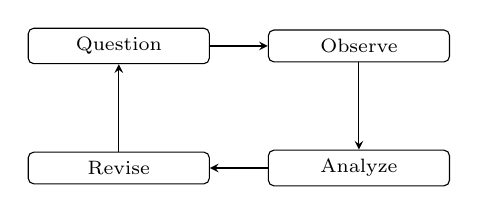
\begin{tikzpicture}[font=\scriptsize, >=stealth, node distance=1.55cm]
\node[draw, rounded corners=2pt, align=center, minimum width=2.3cm] (q) {Question};
\node[draw, rounded corners=2pt, align=center, right of=q, xshift=1.5cm, minimum width=2.3cm] (o) {Observe};
\node[draw, rounded corners=2pt, align=center, below of=o, minimum width=2.3cm] (a) {Analyze};
\node[draw, rounded corners=2pt, align=center, left of=a, xshift=-1.5cm, minimum width=2.3cm] (r) {Revise};
\draw[->] (q) -- (o);
\draw[->] (o) -- (a);
\draw[->] (a) -- (r);
\draw[->] (r) -- (q);
\end{tikzpicture}
\end{adjustbox}
\end{center}

The loop can last seven days, seven months, seven years, or longer. That is not waste. It is the brain being reshaped by a persistent demand for better explanation.

\section*{Excellence as a Necessity}

There is a famous saying: excellence is a habit.

The sentence is correct, but it becomes sharper if we translate it into the language of this chapter:

\begin{quote}
Excellence is what happens when doing one's best becomes a necessity.
\end{quote}

To some people, good enough is not enough. They do not merely want a task finished. They want to know whether it was done as well as they could do it. They may still fail. They may still have limits. But the standard inside them is not casual.

For others, excuse-making is the stronger necessity. When difficulty appears, they immediately need a reason to stop. The mind searches with impressive speed: the environment was unfair, the timing was wrong, the teacher was poor, the tool was missing, the family background was limiting, the market was strange, the body was tired, the age was wrong. Some of these explanations may contain truth. But the function is not truth-seeking. The function is permission.

This too is a kind of drive. It is just pointed in the wrong direction.

A useful interview question is:

\begin{quote}
In what area have you ever been first, or the best, even locally or temporarily?
\end{quote}

The scale does not need to be grand. First in a small team. Best in a class. Best at a narrow craft. First in a local competition. Best among peers at one measurable thing. The point is not vanity. The point is experience. A person who has once pursued the best version of his own work knows something that cannot be fully explained to someone who has never cared.

A strong person often has three marks:

\begin{enumerate}
\item He has the obsession to be first or best in some domain.
\item He has at least one lived experience of reaching that standard.
\item He has reflected on that experience enough to repeat the pattern elsewhere.
\end{enumerate}

Without such experience, mediocrity becomes normal. The danger is not immediate failure. The danger is becoming used to the absence of excellence. After enough years, a person may no longer feel pain when he does not improve.

\section*{Waiting Is Usually an Excuse}

One of the most common excuses is waiting.

When I am older, I will begin. When the company improves, I will begin. When I have more money, I will begin. When I meet the right people, I will begin. When I finish this busy period, I will begin. When conditions are perfect, I will begin.

Some waiting is real. Law, health, duty, and timing can impose genuine constraints. But most waiting is not constraint. It is disguise.

Age does not automatically produce ability. A person can be thirty and unprepared, forty and unprepared, fifty and unprepared. Time passing is not growth. Time invested under pressure, feedback, reflection, and correction can become growth. Time merely endured becomes age.

If something is a true necessity, waiting becomes costly. A person does not wait calmly while an important part of life is starving. He begins awkwardly. He begins before he is ready. He begins because not beginning hurts more than beginning badly.

No success worth having can be waited into existence.

\section*{Correct and Incorrect Necessities}

Necessity itself is not always good. Human beings can turn many poor things into necessities.

Some people need to complain. If they do not complain, they feel blocked. Once they complain, they feel temporarily emptied, but nothing improves. Some people need to live in the past. They repeatedly tell stories of former glory, former fairness, former opportunity, or former suffering. The past becomes their emotional home, and the future receives no investment. Some people need approval. Some need comfort. Some need resentment. Some need to prove that effort is useless, because that belief protects them from the shame of not trying.

This is why the phrase must be precise:

\begin{quote}
Correct necessity is the source of useful self-drive.
\end{quote}

Incorrect necessity also drives behavior, but toward decay. The person is not without energy. He may spend great energy defending excuses, repeating complaints, protecting face, or staying comfortable. The tragedy is that the drive is real but misallocated.

Wealth freedom depends on correcting this allocation. Attention, time, skill, and capital all follow what feels necessary. If comfort is necessary, attention will serve comfort. If face is necessary, time will serve performance. If consumption is necessary, capital will leak. If analysis, growth, patience, and excellence become necessary, the same person begins to compound differently.

\section*{The Brain Is Being Shaped}

Modern neuroscience has made one conclusion difficult to ignore: the brain is plastic. It is not fixed in the crude way people once imagined. Practice changes it. Repeated attention changes it. Habits change it. The environment shapes it, but so does self-directed behavior.

This gives the idea of necessity a physical seriousness. A chosen necessity is not only a slogan. It changes what the person notices, what he repeats, what he tolerates, what he cannot tolerate, and what he practices. Over time, those repetitions reshape the mind that performs them.

The mechanism is plain enough:

\begin{quote}
Necessity directs attention. Attention directs repetition. Repetition reshapes ability. Ability changes life.
\end{quote}

So the deepest form of self-drive is not shouting at oneself to work harder. It is choosing the right necessity so that attention returns to the work again and again.

A person who truly needs analysis will keep analyzing. A person who truly needs reading will keep reading. A person who truly needs excellence will keep improving. A person who truly needs freedom will learn to accumulate skill, capital, judgment, and patience. He will not do it perfectly. But he will keep returning, because the need has become part of him.

\section*{An Exercise in Missing Necessity}

List the skills you have wanted for years but never acquired.

Do not make the list elegant. Make it complete. Languages, writing, health, investing, sales, coding, speaking, design, accounting, negotiation, teaching, management, emotional control, attention control, anything.

Then examine each item with one question:

\begin{quote}
What necessity is missing?
\end{quote}

Perhaps the skill has no real use in your life. Perhaps you admire the identity more than the practice. Perhaps passing a test replaced using the tool. Perhaps comfort is still more necessary than growth. Perhaps approval is more necessary than truth. Perhaps waiting is more necessary than beginning. Perhaps the skill would matter only in a future you have not made vivid enough.

For each skill, design a small but real use. Do not design a fantasy. Design a daily or weekly demand.

Read one original source instead of a summary. Write one public note instead of privately admiring writing. Track one investment decision instead of merely consuming market opinion. Sell one small thing instead of studying sales forever. Ask one better question in a meeting instead of thinking silently afterward. Replace one complaint with one analysis. Replace one plan to start later with one action today.

The point is not drama. The point is insertion. Insert the skill into life until life begins to ask for it.

Self-drive grows when the mind recognizes that the work is no longer optional. The right necessities make a person difficult to stop. They reshape his brain, his habits, his standards, and eventually his fate.
